\documentclass[portrait]{xebaposter}

%\usepackage[vlined]{algorithm2e}
\usepackage{times}
\usepackage{calc}
\usepackage{url}
\usepackage{amsmath}
\usepackage{amssymb}
\usepackage{relsize}
\usepackage{multirow}
\usepackage{booktabs}
\usepackage{graphicx}
\usepackage{multicol}
%\usepackage[T1]{fontenc}
\usepackage{ae}
\usepackage{wrapfig}
\graphicspath{{images/}}

%\usepackage{geometry}
%\geometry{papersize={90cm,170cm},verbose=ture,reset}
 %%%%%%%%%%%%%%%%%%%%%%%%%%%%%%%%%%%%%%%%%%%%%%%%%%%%%%%%%%%%%%%%%%%%%%%%%%%%%%%%
 %%%% Some math symbols used in the text
 %%%%%%%%%%%%%%%%%%%%%%%%%%%%%%%%%%%%%%%%%%%%%%%%%%%%%%%%%%%%%%%%%%%%%%%%%%%%%%%%
 % Format 
% \newcommand{\RotUP}[1]{\begin{sideways}#1\end{sideways}}


 %%%%%%%%%%%%%%%%%%%%%%%%%%%%%%%%%%%%%%%%%%%%%%%%%%%%%%%%%%%%%%%%%%%%%%%%%%%%%%%%
 % Multicol Settings
 %%%%%%%%%%%%%%%%%%%%%%%%%%%%%%%%%%%%%%%%%%%%%%%%%%%%%%%%%%%%%%%%%%%%%%%%%%%%%%%%
% \setlength{\columnsep}{0.7em}
% \setlength{\columnseprule}{0mm}


 %%%%%%%%%%%%%%%%%%%%%%%%%%%%%%%%%%%%%%%%%%%%%%%%%%%%%%%%%%%%%%%%%%%%%%%%%%%%%%%%
 % Save space in lists. Use this after the opening of the list
 %%%%%%%%%%%%%%%%%%%%%%%%%%%%%%%%%%%%%%%%%%%%%%%%%%%%%%%%%%%%%%%%%%%%%%%%%%%%%%%%
 \newcommand{\compresslist}{%
 \setlength{\itemsep}{1pt}%
 \setlength{\parskip}{0pt}%
 \setlength{\parsep}{0pt}%
 }

%% Begin of Document
%%%%%%%%%%%%%%%%%%%%%%%%%%%%%%%%%%%%%%%%%%%%%%%%%%%%%%%%%%%%%%%%%%%%%%%%%%%%%
\begin{document}

%%%%%%%%%%%%%%%%%%%%%%%%%%%%%%%%%%%%%%%%%%%%%%%%%%%%%%%%%%%%%%%%%%%%%%%%%%%%%
%% Here starts the poster
%%---------------------------------------------------------------------------
%% Format it to your taste with the options
%%%%%%%%%%%%%%%%%%%%%%%%%%%%%%%%%%%%%%%%%%%%%%%%%%%%%%%%%%%%%%%%%%%%%%%%%%%%%
      \definecolor{silver}{cmyk}{0,0,0,0.3}
      \definecolor{yellow}{cmyk}{0,0,0.9,0.0}
      \definecolor{reddishyellow}{cmyk}{0,0.22,1.0,0.0}
      \definecolor{black}{cmyk}{0,0,0.0,1.0}
      \definecolor{darkYellow}{cmyk}{0,0,1.0,0.5}
      \definecolor{darkSilver}{cmyk}{0,0,0,0.1}

      \definecolor{lightyellow}{cmyk}{0,0,0.3,0.0}
      \definecolor{lighteryellow}{cmyk}{0,0,0.1,0.0}
      \definecolor{lighteryellow}{cmyk}{0,0,0.1,0.0}
      \definecolor{lightestyellow}{cmyk}{0,0,0.05,0.0}

      \begin{poster}%
      % Poster Options
      {
      eyecatcher=false,
      % Color style
      bgColorOne=darkSilver,
      bgColorTwo=lighteryellow,
      borderColor=reddishyellow,
      headerColorOne=yellow,
      headerColorTwo=reddishyellow,
      headerFontColor=black,
      boxColorOne=lightyellow,
      boxColorTwo=darkSilver,
      % Format of textbox
      textborder=faded,
      % Format of text header
      headerborder=open,
      headerheight=0.1\textheight,
      headershape=rectangle,
      headershade=shadetb,
%      headerfont=\Large, %Sans Serif
      boxshade=shadeLR,
%      background=plain,
      linewidth=2pt,
%      grid=true,
      }
 % Eye Catcher
 {
      
\includegraphics[width=0.08\linewidth]{logo}
%      \includegraphics[width=0.08\linewidth]{track_frame_00450_06}
%      \includegraphics[width=0.08\linewidth]{track_frame_04999_06}
 }
 % Title
 {Parallel Nonlinear Analysis of Weighted Brain's Gray and White Matter Images for Alzheimer's Dementia Diagnosis}
 % Authors
 {\large Seiied-Mohammad-Javad~Razavian, Meysam Torabi, and Kio Kim \\%[1em]
 {\normalsize\texttt{javad@cs.sharif.edu, torabi@berkeley.edu, kio.kim@ucsf.edu}}}
 % University logo
 {
\begin{tabular}{r}
    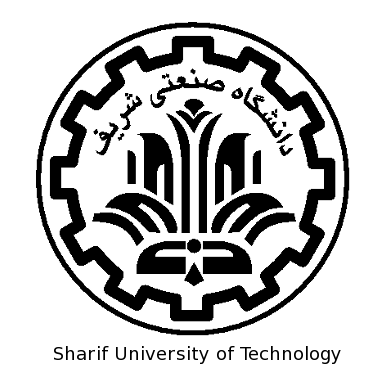
\includegraphics[height=0.07 \textheight]{shariflogo}\\
\end{tabular}
 }

%%%%%%%%%%%%%%%%%%%%%%%%%%%%%%%%%%%%%%%%%%%%%%%%%%%%%%%%%%%%%%%%%%%%%%%%%%%%%%
%%% Now define the boxes that make up the poster
%%%---------------------------------------------------------------------------
%%% Each box has a name and can be placed absolutely or relatively.
%%% The only inconvenience is that you can only specify a relative position 
%%% towards an already declared box. So if you have a box attached to the 
%%% bottom, one to the top and a third one which should be inbetween, you 
%%% have to specify the top and bottom boxes before you specify the middle 
%%% box.
%%%%%%%%%%%%%%%%%%%%%%%%%%%%%%%%%%%%%%%%%%%%%%%%%%%%%%%%%%%%%%%%%%%%%%%%%%%%%%

%%%%%%%%%%%%%%%%%%%%%%%%%%%%%%%%%%%%%%%%%%%%%%%%%%%%%%%%%%%%%%%%%%%%%%%%%%%%%%
%  \headerbox{Abstract}{name=abstract,column=0,row=0,span=1}{
%%%%%%%%%%%%%%%%%%%%%%%%%%%%%%%%%%%%%%%%%%%%%%%%%%%%%%%%%%%%%%%%%%%%%%%%%%%%%%%
%We are proposing a novel approach using T1-weighted and T2-weighted Magnetic Resonance Images (MRI's) of brain. Since T1-weighted images and T2-weighted images have inherent physical differences, we extracted some specific features from each. Then the variations of the relevant eigenvalues of the extracted features were tracked to pick up the most informative ones. The final features were assigned to two parallel systems to be nonlinearly categorized. The dataset includes 60 T1-weighted images and 60 T2-weighted images of normal and abnormal cases.
%  }
 
 %%%%%%%%%%%%%%%%%%%%%%%%%%%%%%%%%%%%%%%%%%%%%%%%%%%%%%%%%%%%%%%%%%%%%%%%%%%%%%
   \headerbox{Introduction}{name=introduction,column=0,row=0}{
 %%%%%%%%%%%%%%%%%%%%%%%%%%%%%%%%%%%%%%%%%%%%%%%%%%%%%%%%%%%%%%%%%%%%%%%%%%%%%%
%AD disease destroys the nervous system and defects the temporal lobe and parietal lobe of the brain. 

%\begin{wrapfigure}[10]{r}{.72\textwidth}
%\centering
%{\includegraphics[scale=.9]{Maghz}}
%\end{wrapfigure}
We introduce a novel method for Alzheimer's dementia diagnosis.
Our focus is on analysis of MRI because of its high resolution in brain tissues.% which includes normal and abnormal cases.
We believe that the tissue analysis can be a reliable tool to diagnose various diseases. The novelty of this work is using both T1 and T2 images simultaneously after they are optimally weighted.
   }

 %%%%%%%%%%%%%%%%%%%%%%%%%%%%%%%%%%%%%%%%%%%%%%%%%%%%%%%%%%%%%%%%%%%%%%%%%%%%%%
   \headerbox{Phase II: core processing}{name=phase2,column=1,span=1}{
 %%%%%%%%%%%%%%%%%%%%%%%%%%%%%%%%%%%%%%%%%%%%%%%%%%%%%%%%%%%%%%%%%%%%%%%%%%%%%%
We extracted features which can capture the properties of the brain tissue using Gray-Level Co-occurrence Matrix (GLCM) which helps scan the tissue in order to give a sense of how the relationship between different pixels of an image is.% \cite{BeDeTo}, 
%\textbf{Neighborhood definition and calculating GLC matrix}%

\begin{wrapfigure}{r}{.6\textwidth}
\centering
  \vspace{-10pt}
{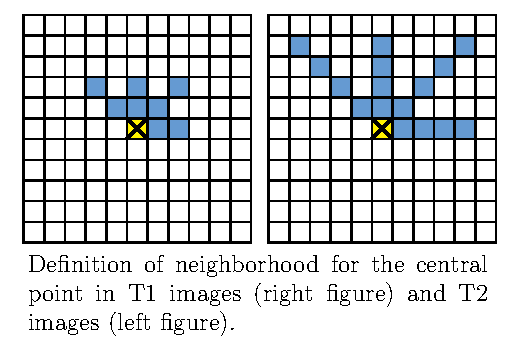
\includegraphics[scale=.5]{fig3}}
  \vspace{-20pt}
%\caption{\scriptsize Right figure shows the definition of neighborhood for the central point in T1 images while the left figure shows the definition of the neighborhood for T2. As it can be obviously seen in the figure, the neighborhood defined for T1 covers more detail.} 
\label{fig3}
\end{wrapfigure}

Considering the fact that AD defects the white and gray regions of brain more than its black and marginal regions, and also since T1-weighted has more medical data of white and gray regions than T2-weighted images, we believe that T1 images have more data than T2 images, thus we define neighborhood of T1 and T2 differently.

%\textbf{Extraction of statistical features from GLC matrices}
The desired Statistical features are as follows:
1) Energy,
2) Contrast,
3) Homogeneity, and
4) Correlation

%To calculate correlation, two following parameters initially are calculated:
%in which elements of GLC matrix are shown with the symbol C(i, j) and the number of gray-levels with N.

Correlation in the GLC matrix:
\begin{align*}
f_1 &= \frac{HXY-HXY1}{max\{HX,HY\}}\\
f_2 &= \sqrt{1-\exp\{-2(HXY2-HXY)\}} 
\end{align*}
%in which, $HX$ and $HY$ are entropy of $C_x$ and $C_y$ respectively, and $HXY$, $HXY1$ and $HXY2$ are defined as follows, respectively:
{\scriptsize 
\centerline{\begin{minipage}{.95\textwidth}
C(i, j) is an element of GLC matrix and N is number of gray-levels.
\end{minipage}}
\vspace{-.5mm}
$$\begin{array}{l}
 C_x(i) =\sum_{j=1}^N C(i,j), \quad C_y(i)=\sum_{i=1}^N C(i,j)\\
  HXY = -\sum_{i=1}^N\sum_{j=1}^N C(i,j) \log\{C(i,j)\}\\
  HXY1 = -\sum_{i=1}^N\sum_{j=1}^N C(i,j) \log\{C_x(i)\times C_y(j)\}\\
  HXY2 = -\sum_{i=1}^N\sum_{j=1}^N C_x(i)\times C_y(j) \log\{C_x(i)\times C_y(j)\}\\
\end{array}$$
}

4*16 features from T1 and 4*8 features from T2 are extracted.
}

 %%%%%%%%%%%%%%%%%%%%%%%%%%%%%%%%%%%%%%%%%%%%%%%%%%%%%%%%%%%%%%%%%%%%%%%%%%%%%%
%   \headerbox{Phase III: Feature Analysis}{name=phase3,column=2,span=1,row=0}{
   \headerbox{Feature Extraction}{name=phase3,column=2,span=1,row=0}{
 %%%%%%%%%%%%%%%%%%%%%%%%%%%%%%%%%%%%%%%%%%%%%%%%%%%%%%%%%%%%%%%%%%%%%%%%%%%%%%
We reduce two vectors, one for T1 images and another one for T2 images that using PCA. % for extracting the main components.
%Our simulation results are demonstrated in Figure~\ref{fig4}, showing the last 20 eigenvalues of both T1 images and T2 images. Other eigenvalues are not displayed, since, as the figure implies, they are almost zero. Thus, 
We chose 19 first eigenvalues with the largest values for T1 image, and also 17 eigenvalues with the largest values  for T2 images.

%\centering
\centerline{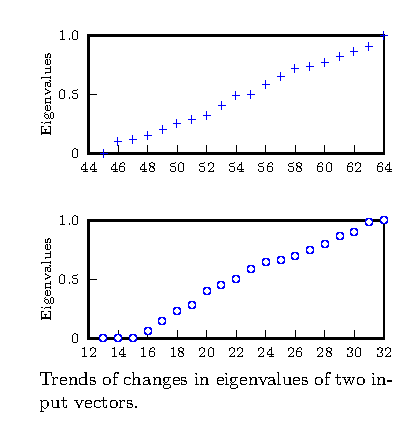
\includegraphics[scale=1.1,height=7cm]{fig4}}
%\caption{Trends of changes in eigenvalues of two input vectors.} 
%\label{fig4}
%\end{figure}
 }

 %%%%%%%%%%%%%%%%%%%%%%%%%%%%%%%%%%%%%%%%%%%%%%%%%%%%%%%%%%%%%%%%%%%%%%%%%%%%%%
%   \headerbox{Phase IV:  Discrimination }{name=phase4,column=2,span=1,below=phase3}{
   \headerbox{Discrimination }{name=phase4,column=2,span=1,below=phase3}{   
 %%%%%%%%%%%%%%%%%%%%%%%%%%%%%%%%%%%%%%%%%%%%%%%%%%%%%%%%%%%%%%%%%%%%%%%%%%%%%%
Two feed-forward neural networks are tuned and used with 19 and 17 inputs for analysis of T1 and T2 images respectively. Both networks have a hidden layer with 10 nodes equipped with Sigmoid transfer function.

We multiply the first neural network's output by weighting factor 0.63, and also multiply the second neural network's output by weighting factor 0.37, that were initialized and determined during the training of the classifier system. 


}

 %%%%%%%%%%%%%%%%%%%%%%%%%%%%%%%%%%%%%%%%%%%%%%%%%%%%%%%%%%%%%%%%%%%%%%%%%%%%%%
   \headerbox{Results }{name=results,column=1,span=2,below=phase2}{
 %%%%%%%%%%%%%%%%%%%%%%%%%%%%%%%%%%%%%%%%%%%%%%%%%%%%%%%%%%%%%%%%%%%%%%%%%%%%%%
\begin{multicols}{2}
In order to give a more clear measure of the performance of the classifier system, consisting of two parallel neural networks, the right-top figure illustrates an ROC graph. 

However, higher accuracies in separation of training data can cause a better result in our database, but this increases the number of layers and nodes of the neural networks which may lead to overtraining of the system and thus, it may reduce the classification accuracy of test images. Therefore, we believe that the response shown here is an optimal one.

%We aware of similar works of other researchers (e.g. \cite{WaRoCoSpBaGaDoChSe,FrFo}) in which they obtained better results, but We try to increase the speed of process to have a real-time classifier system.

In the future research, we try to, in addition
to improving the diagnosis of AD, produce initially independent features in
order to increase the speed of process to have a real-time
classifier system.

\centerline{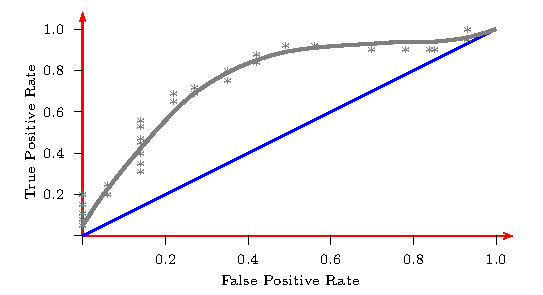
\includegraphics[scale=.7]{fig6}}
%\caption{An ROC graph corresponding to classifier's responses shows the accuracy of the proposed AD diagnosis system.} 
\centerline{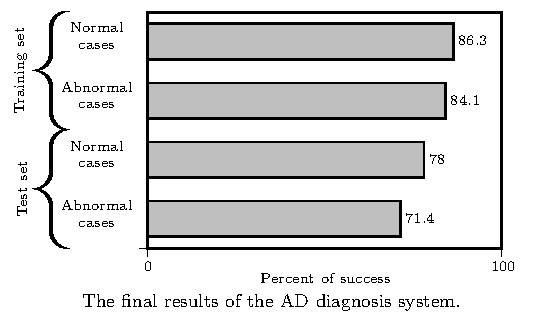
\includegraphics[scale=.7]{fig5}}
%\caption{The final result of the AD diagnosis system.} 

\end{multicols}
}


 %%%%%%%%%%%%%%%%%%%%%%%%%%%%%%%%%%%%%%%%%%%%%%%%%%%%%%%%%%%%%%%%%%%%%%%%%%%%%%
%   \headerbox{Related Works}{name=relatedworks,column=0,below=introduction}{
% %%%%%%%%%%%%%%%%%%%%%%%%%%%%%%%%%%%%%%%%%%%%%%%%%%%%%%%%%%%%%%%%%%%%%%%%%%%%%%
%A review of the works done during the last 20 years :
%\begin{itemize}
%\compresslist
%	\item brain atrophy %\cite{WaRoCoSpBaGaDoChSe}
%	\item number and size of senile plaques in the brain %\cite{HaHoDe}
%	\item deformation of the brain structure %\cite{MaPe}
%	\item bio-signal processing  %\cite{HaPeGaMo}.
%	\item medical image processing and analysis
%\begin{itemize}
%	\compresslist
%		\item 	microscopic methods
%		\item 	macroscopic methods
%	\end{itemize}
%\end{itemize}
%{\scriptsize (see paper for references.)}
%}

%%%%%%%%%%%%%%%%%%%%%%%%%%%%%%%%%%%%%%%%%%%%%%%%%%%%%%%%%%%%%%%%%%%%%%%%%%%%%%
   \headerbox{Brain Images Dataset}{name=imagedataset,column=0,span=1,below=introduction}{
 %%%%%%%%%%%%%%%%%%%%%%%%%%%%%%%%%%%%%%%%%%%%%%%%%%%%%%%%%%%%%%%%%%%%%%%%%%%%%%
\begin{itemize}
\compresslist
	\item 120 MRI's (including T1 and T2 images) for different cross-sections of the brain
	\item 52 images belong to the normal control group while the rest belongs to AD patients. 
	\item Half of the images is T1 and the other half is T2.
	\item 60 percent of the images is used for training, and the rest is reserved to test and control the algorithm. 
	\item Images dataset: The Whole Brain Atlas. Available on \url{http://www.med.harvard.edu/AANLIB/home.html}
\end{itemize}
  }

  %%%%%%%%%%%%%%%%%%%%%%%%%%%%%%%%%%%%%%%%%%%%%%%%%%%%%%%%%%%%%%%%%%%%%%%%%%%%%%
   \headerbox{Disease Diagnosis Method}{name=ddm,column=0,span=1,below=imagedataset}{
 %%%%%%%%%%%%%%%%%%%%%%%%%%%%%%%%%%%%%%%%%%%%%%%%%%%%%%%%%%%%%%%%%%%%%%%%%%%%%%
\centerline{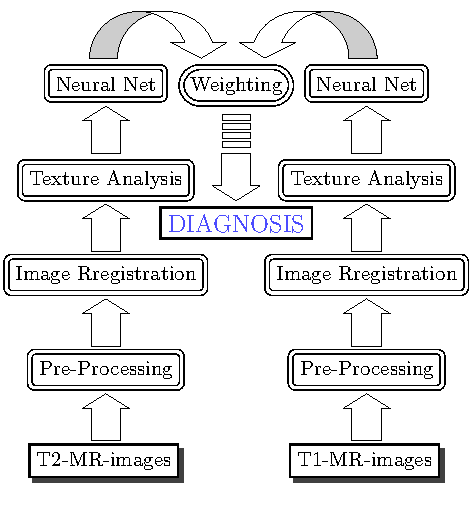
\includegraphics[scale=.7,width=.9\textwidth,height=6cm]{fig1}}
    }

 %%%%%%%%%%%%%%%%%%%%%%%%%%%%%%%%%%%%%%%%%%%%%%%%%%%%%%%%%%%%%%%%%%%%%%%%%%%%%%
   \headerbox{Phase I: preprocessing}{name=phase1,column=0,span=1,below=ddm}{
 %%%%%%%%%%%%%%%%%%%%%%%%%%%%%%%%%%%%%%%%%%%%%%%%%%%%%%%%%%%%%%%%%%%%%%%%%%%%%%
Removing irrelevant information:% that does not help the algorithm detect AD:
\begin{enumerate}
\compresslist
	\item marginal parts of the images.
	\item background.
	\item other parts of brain, e.g. parts of eyes.
\end{enumerate}
%\subsubsection*{Registration}
We registered each image on its corresponding image as precisely as possible using 10 landmarks. The landmarks are located and placed on those points of the brain which are geometrically and anatomically more important. %\cite{YuXiBeLiZhGuDeJuWo}. 
%\cite{ToMoVaRaDeRaTaFa}.
%(Figure~\ref{fig2}). 
Registration includes %two stages of interpolation: 
1) pixel position interpolation and 2) gray-level interpolation. For performing interpolation process, radial basis function $r^2 \log r^2$ is used. %\cite{ToMoVaRaDeRaTaFa}. 
The affine terms have not been used in the proposed algorithm, since the results were already satisfactory.

\centerline{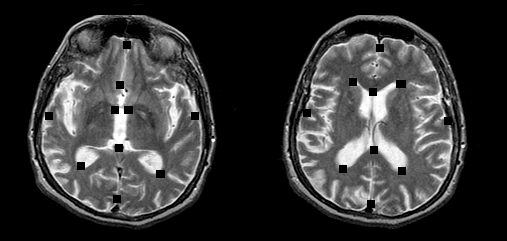
\includegraphics[scale=.34]{fig2}}
\centerline{\begin{minipage}{.8\textwidth}
\scriptsize Two samples of cross-sections of brain which are marked with 10 landmarks.
\end{minipage}}
%{\scriptsize Two samples of cross-sections of brain which are marked with 10 landmarks.} 
%\label{fig2}

}
    
%%%%%%%%%%%%%%%%%%%%%%%%%%%%%%%%%%%%%%%%%%%%%%%%%%%%%%%%%%%%%%%%%%%%%%%%%%%%%%%
%   \headerbox{Funding}{name=funding,column=1,span=2,above=bottom}{
% %%%%%%%%%%%%%%%%%%%%%%%%%%%%%%%%%%%%%%%%%%%%%%%%%%%%%%%%%%%%%%%%%%%%%%%%%%%%%%
%	This work is entirely done at Sharif University of Technology, Tehran, Iran.
%  }
 
 %%%%%%%%%%%%%%%%%%%%%%%%%%%%%%%%%%%%%%%%%%%%%%%%%%%%%%%%%%%%%%%%%%%%%%%%%%%%%%
   \headerbox{References}{name=references,column=1,span=2,below=results}{
 %%%%%%%%%%%%%%%%%%%%%%%%%%%%%%%%%%%%%%%%%%%%%%%%%%%%%%%%%%%%%%%%%%%%%%%%%%%%%%
     \smaller
     
     \bibliographystyle{ieee}
     \renewcommand{\section}[2]{\vskip 0.05em}
       \begin{thebibliography}{1}\itemsep=-0.01em
       \setlength{\baselineskip}{0.4em}

%       \bibitem{amberg07:nicp}
%       B.~Amberg, A.~Blake, T.~Vetter
%       \newblock On Compositional Image Alignment with an Application to Activce Appearance Models
%       \newblock In {\em CVPR'09}, 2009.
       \bibitem{}
       M. Torabi, H. Moradzadeh, R. Vaziri, S. M. J. Razavian, R. Dehestani
	Ardekani, M. Rahmandoost, A. Taalimi, and E. Fatemizadeh, ``Development 
	of Alzheimer's Disease Recognition Using Semiautomatic
	Analysis of Statistical Parameters Based on Frequency Characteristics
	of Medical Images,'' in \emph{Proc. of IEEE Int. Conf. Signal Proc. \&
	Communication}, Nov 2007, pp. 868--871.
       \bibitem{}
	 M. Torabi, R. Dehestani Ardekani, and E. Fatemizadeh, ``Discriminationnation 
	 between Alzheimer's Disease and Control Group in MR-Images Based 
	 on Texture Analysis Using Artificial Neural Network,''
	 in \emph{Proc. of Int. Conf. Bio. \& Pharm. Eng.}, Dec 2006, pp. 79--83.

       \end{thebibliography}
   }
 
 %%%%%%%%%%%%%%%%%%%%%%%%%%%%%%%%%%%%%%%%%%%%%%%%%%%%%%%%%%%%%%%%%%%%%%%%%%%%%%
   \headerbox{Acknowledgment}{name=ack,column=1,span=2,below=references}{
 %%%%%%%%%%%%%%%%%%%%%%%%%%%%%%%%%%%%%%%%%%%%%%%%%%%%%%%%%%%%%%%%%%%%%%%%%%%%%%
 The main concept of this work is inspired by the ideas of the philosopher Majid Jafari-Tabar.
}

\end{poster}%
%
\end{document}
